\documentclass[usenames,dvipsnames,french]{beamer}

\mode<presentation> {

\usetheme{Montpellier}
}

\usepackage{graphicx} % Allows including images
\usepackage[frenchb]{babel}
\usepackage[T1]{fontenc}
\usepackage[utf8]{inputenc}
% \usepackage[demo]{graphicx}
% \usepackage{caption}

\usepackage{subcaption}
% \usepackage{subfig}
% \usepackage{algorithm,algorithmic}
\usepackage{algorithm2e}
\usepackage{listings}
% \usepackage{ntheorem}
\usepackage{booktabs} % Allows the use of \toprule, \midrule and \bottomrule in tables
\setcounter{tocdepth}{2}
\graphicspath{{../../Figures/}}


% exercices comptés
\newcounter{numexos}%Création d'un compteur qui s'appelle numexos
\setcounter{numexos}{0}%initialisation du compteur
\newcommand{\exercice}[1]{%Création d'une macro ayant un paramètre
\addtocounter{numexos}{1}%chaque fois que cette macro est appelée, elle ajoute 1 au compteur numexos
\textcolor{DarkOrchid}{Exercice\,\thenumexos\,:}\,#1%Met en rouge Exercice et la valeur du compteur appelée par \thenumeexos
}
%----------------------------------------------------------------------------------------
%	TITLE PAGE
%----------------------------------------------------------------------------------------

\setbeamertemplate{title page}{
    \centering

    \Large\bfseries
    Machine learning Tek 5: clustering
    

\begin{figure}[!h]
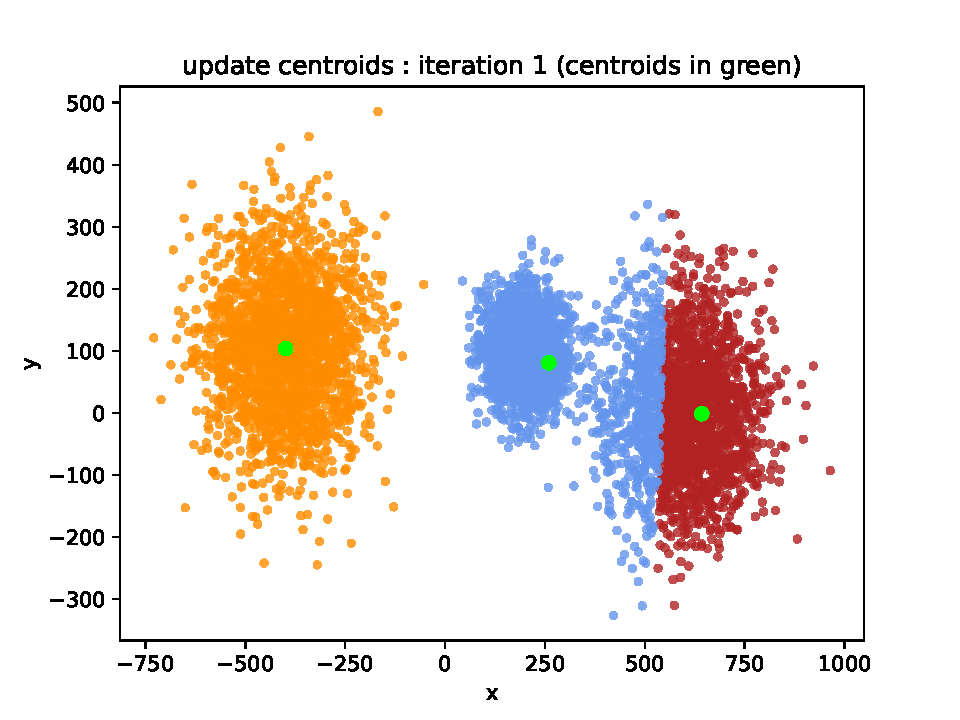
\includegraphics[width=8cm]{it_1_move_centroids}
\end{figure}

    }
\begin{document}

\frame{\titlepage}

\begin{frame}
    \tableofcontents
\end{frame}

\section{Motivation}
\frame{\tableofcontents[currentsection]}

\begin{frame}{Clustering (technical definition)}
    \textbf{{Clustering}}  consists in \textbf{partitioning} the data. $\forall i, x_i\in \mathcal{X}^n$.
    \begin{equation}
	D_n = \{(x_i)_{i\in [1, \dots, n]}\}
    \end{equation}

    A \textbf{{partition}} is a set of $K$ subsets $A_k\subset D_n$, such that
    \begin{itemize}
        \item
	    \begin{equation}
		\cup_{k\in [1, \dots, K]}A_k = D_n
	    \end{equation}
	\item 
	    \begin{equation}
		\forall k\neq k', A_k\cap A_{k'} = \emptyset
	    \end{equation}
    \end{itemize}
\end{frame}

\begin{frame}{Partitions}

    \begin{itemize}
	\item \textbf{{Example 1:}} $A$ is the set of even integers, $B$ the set of odd integers. Is $(A, B)$ a partition of $ \mathbb{N} $ ?
	\item \textbf{{Example 2:}} $C$ is the set of multiples of $2$, $D$ the set of multiples of $3$. Is $(C, D)$ a partition of $ \mathbb{N} $ ?
    \end{itemize}
    
\end{frame}

\begin{frame}{Example: partition of data}
    \begin{figure}[htpb]
        \centering
        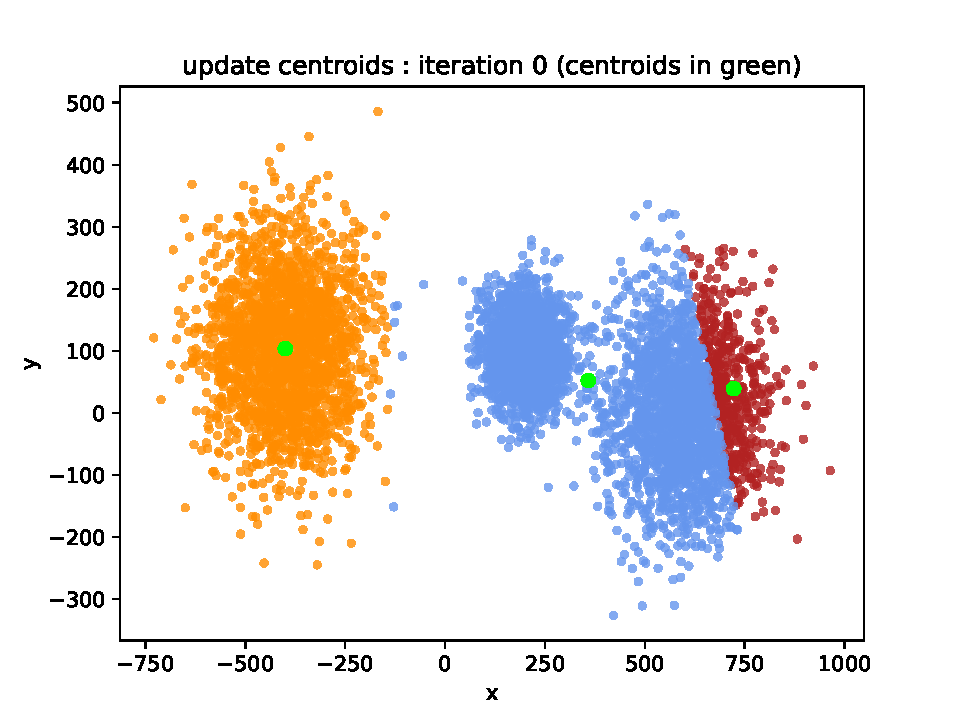
\includegraphics[width=0.7\linewidth]{it_0_move_centroids}
	\caption{In this image, each cluster is represented by a color.}
        \label{fig:it_0_move_centroids}
    \end{figure}
\end{frame}

\begin{frame}{Applications of clustering}
    Example applications:
    \begin{itemize}
	\item spam filtering \cite[]{Sharma2014} 
        \item fake news identification \cite[]{Hosseinimotlagh2018} 
	\item marketing and sales
	\item document analysis \cite[]{Zhao2002} 
	\item traffic classification \cite[]{Woo2007} 
    \end{itemize}

    Some of these applications can be considered to be semi-supervised learning.
\end{frame}

\begin{frame}{Clustering is wide}

    \begin{itemize}
    	\item Applications:
	    \begin{itemize}
	    	\item \url{https://en.wikipedia.org/wiki/Cluster_analysis} 
		\item \url{https://datafloq.com/read/7-innovative-uses-of-clustering-algorithms/} 
	    \end{itemize}

	\item Many clustering algorithms exist !

    \url{https://scikit-learn.org/stable/modules/clustering.html} 


    \end{itemize}

\end{frame}

\section{K-means clustering} % (fold)
\label{sub:subsection_name}

\begin{frame}
\frametitle{K means clustering}
\begin{figure}[!h]
    \centering
    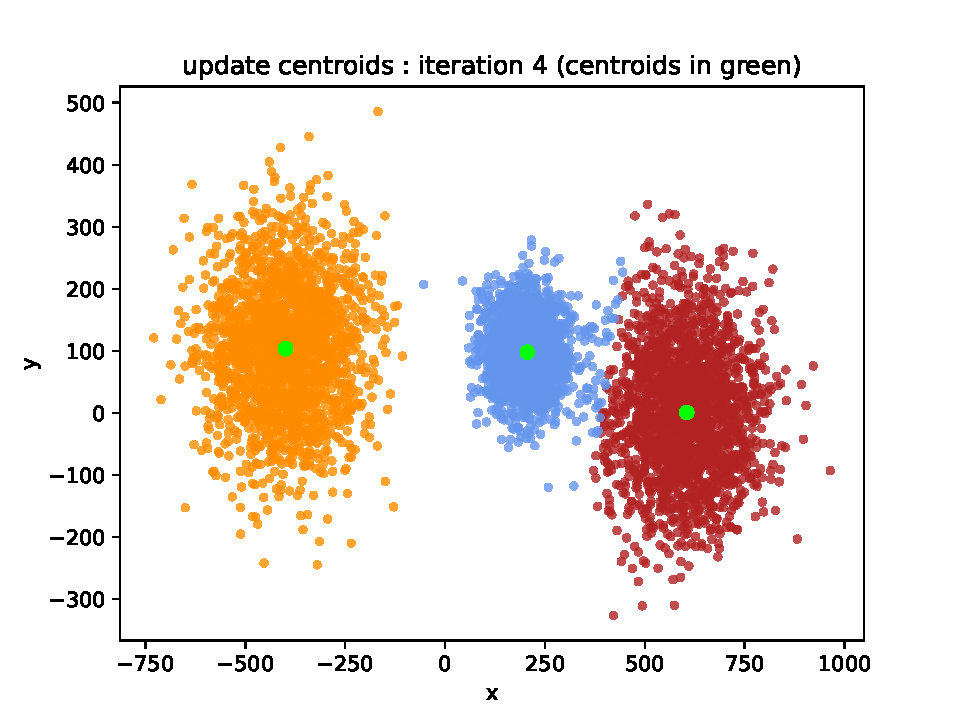
\includegraphics[width=6cm]{it_4_assign_samples_to_centroid}
    \caption{K means clustering}
    \label{figure}
\end{figure}
\end{frame}


\begin{frame}
\frametitle{K-means}
\begin{figure}[!h]
\centering
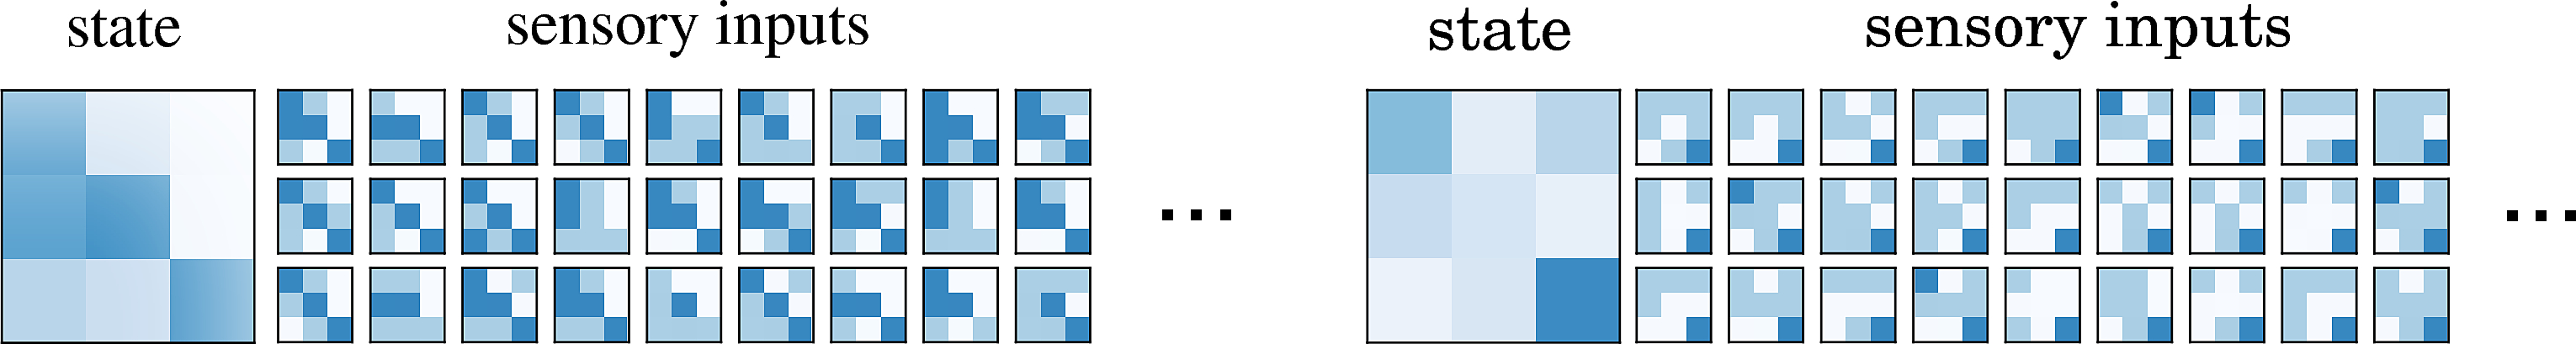
\includegraphics[width=12cm]{fig_kmeans.jpg}
\caption{Other example of k-means clustering, this time in 9 dimensions \cite{LeHir2018}}
\label{figure}
\end{figure}
\end{frame}


\begin{frame}
\frametitle{K-means : Expectation Maximisation algorithm}
\begin{itemize}
	\item Classical Machine Learning algorithm (EM)
	\item Discussion on the drawbacks of the algorithm.
\end{itemize}
\end{frame}

\begin{frame}{K-means clustering}
\exercice{\textbf{Implementing kmeans}}
\addtocounter{numexos}{-1}
\begin{figure}[!h]
\centering
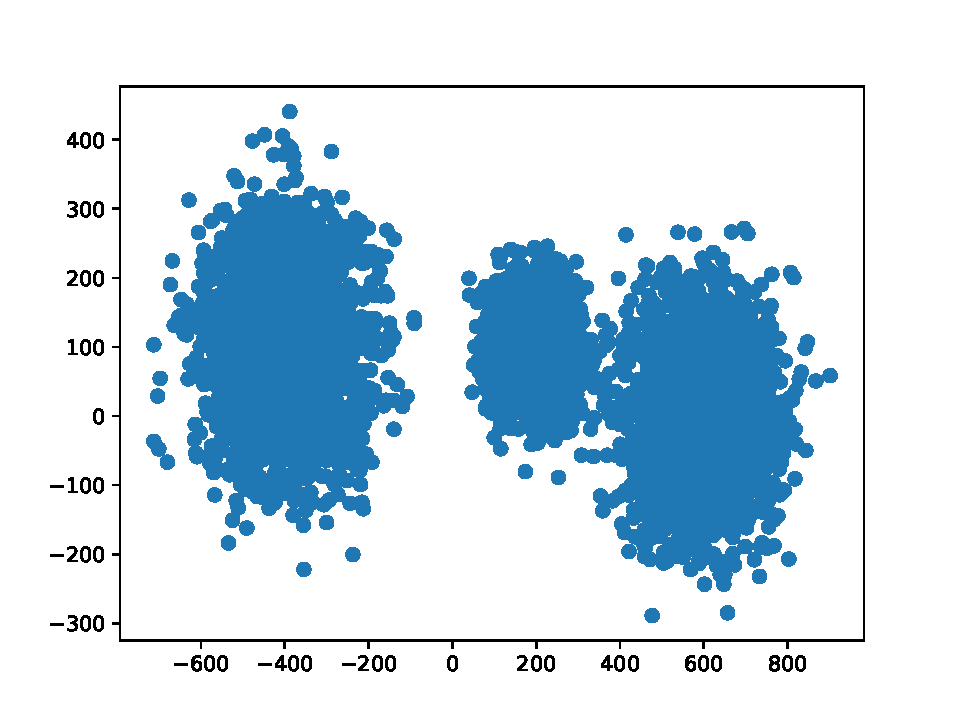
\includegraphics[width=6.5cm]{kmeans_data}
\caption{Data we want to cluster}
\label{figure}
\end{figure}
\end{frame}


\begin{frame}{K-means clustering}
\exercice{\textbf{Implementing k-means}}

\textbf{cd 4\textunderscore clustering/1\textunderscore k\textunderscore means/}.

Edit the \textbf{k\textunderscore means.py} file so that it performs the k-means algorithm, on the example dataset, with $3$ clusters.

You can use for loops or try to directly write the algorithm in a vectorized way.
\end{frame}


\begin{frame}
\frametitle{K-means}
\begin{figure}[!h]
\centering
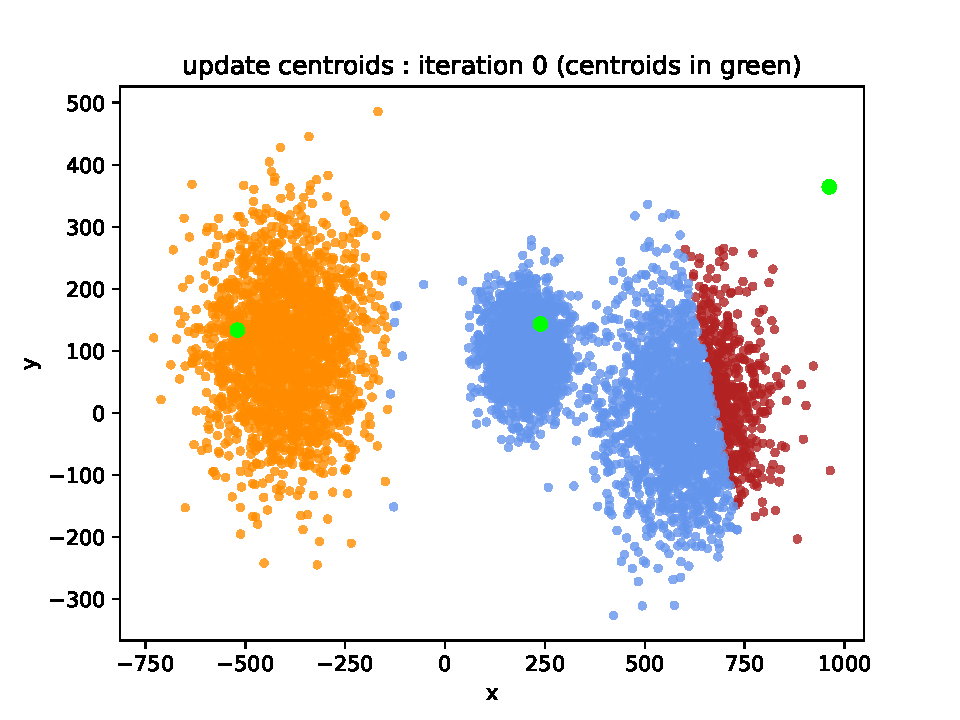
\includegraphics[width=8.5cm]{it_0_assign_samples_to_centroid}
\label{figure}
\end{figure}
\end{frame}

\begin{frame}
\frametitle{K-means}
\begin{figure}[!h]
\centering
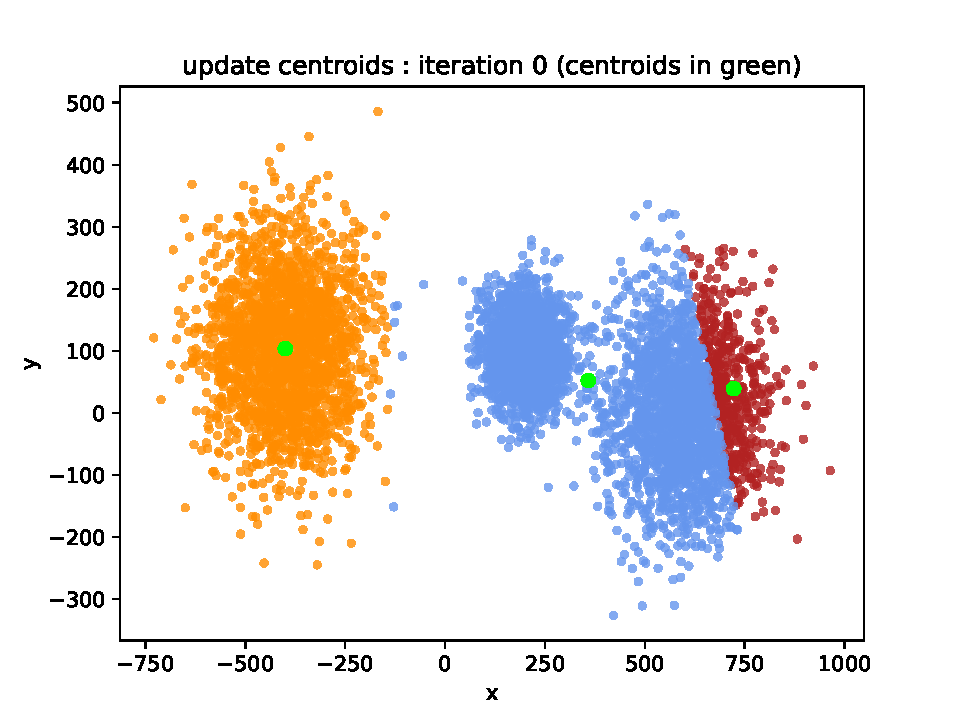
\includegraphics[width=8.5cm]{it_0_move_centroids}
\caption{Centroids 0th iteration}
\label{figure}
\end{figure}
\end{frame}

\begin{frame}
\frametitle{K-means}
\begin{figure}[!h]
\centering
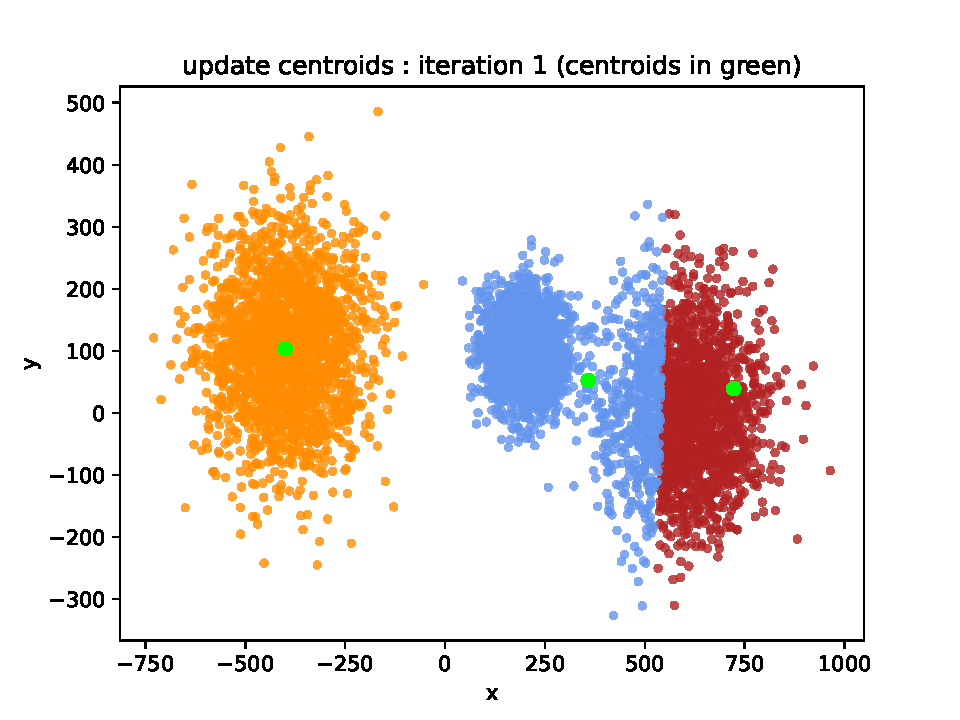
\includegraphics[width=8.5cm]{it_1_assign_samples_to_centroid}
\caption{}
\label{figure}
\end{figure}
\end{frame}

\begin{frame}
\frametitle{K-means}
\begin{figure}[!h]
\centering
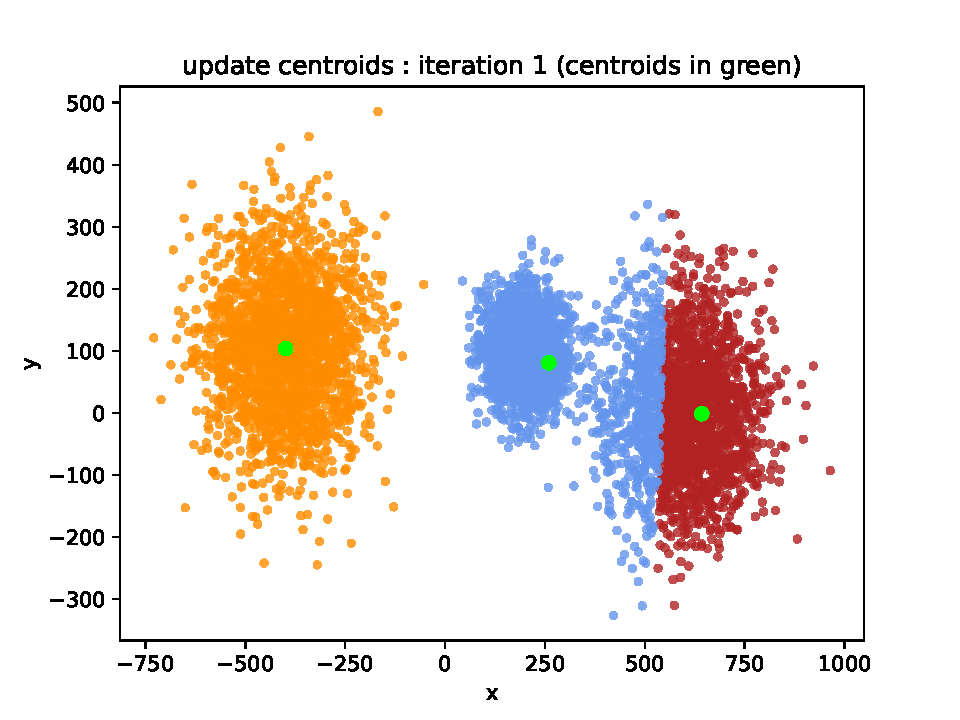
\includegraphics[width=8.5cm]{it_1_move_centroids}
\caption{Centroids 1st iteration}
\label{figure}
\end{figure}
\end{frame}


\begin{frame}
\frametitle{K-means}
\begin{figure}[!h]
\centering
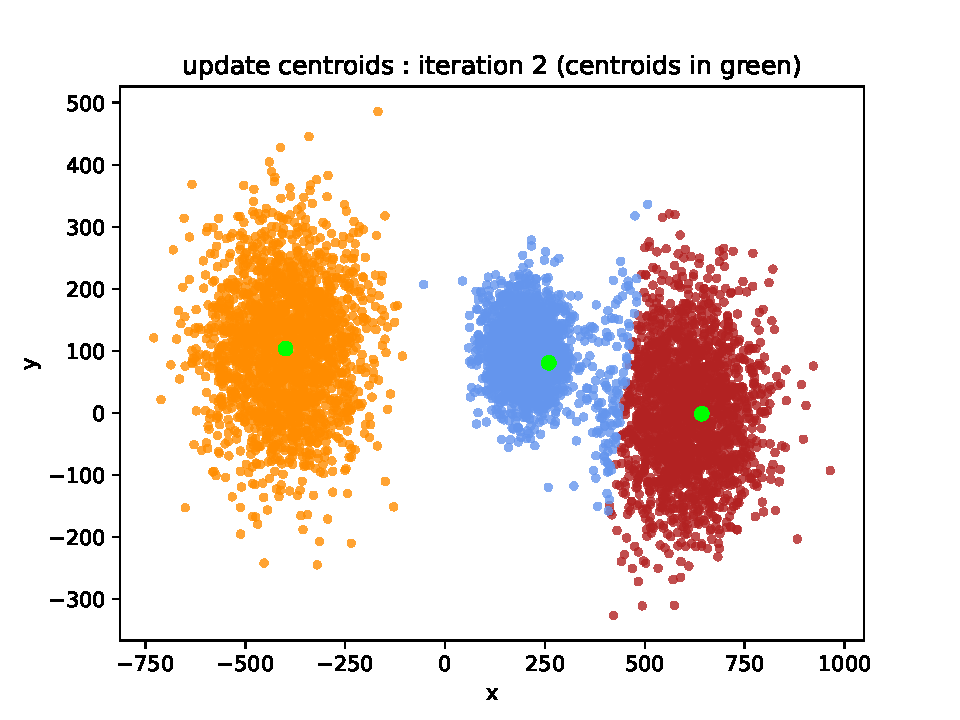
\includegraphics[width=8.5cm]{it_2_assign_samples_to_centroid}
\caption{}
\label{figure}
\end{figure}
\end{frame}

\begin{frame}
\frametitle{K-means}
\begin{figure}[!h]
\centering
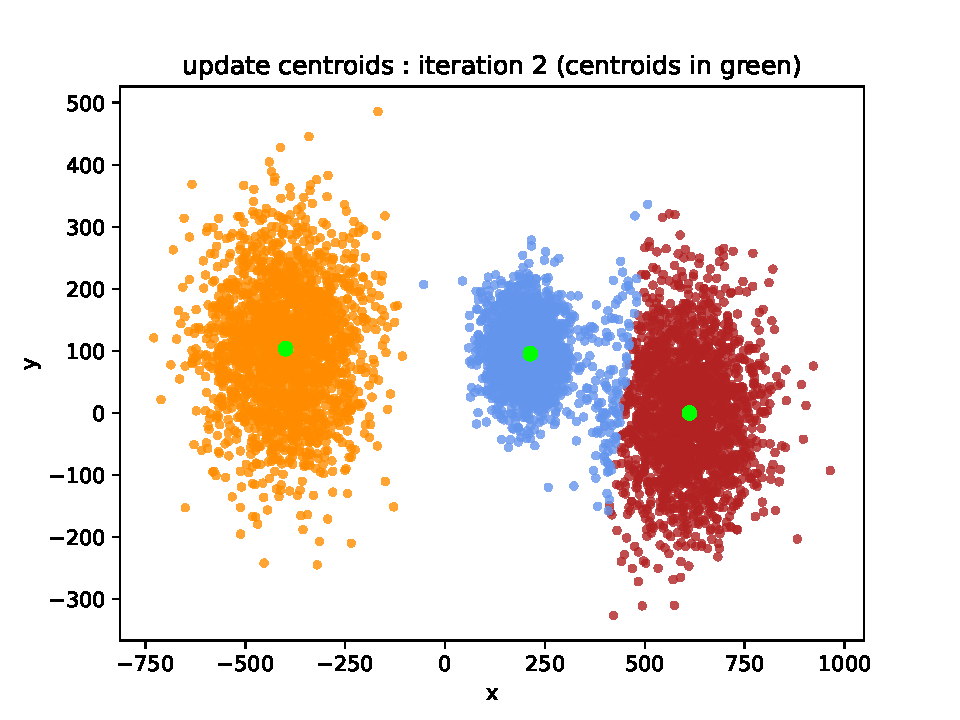
\includegraphics[width=8.5cm]{it_2_move_centroids}
\caption{Centroids 1st iteration}
\label{figure}
\end{figure}
\end{frame}

\begin{frame}
\frametitle{K-means}
\begin{figure}[!h]
\centering
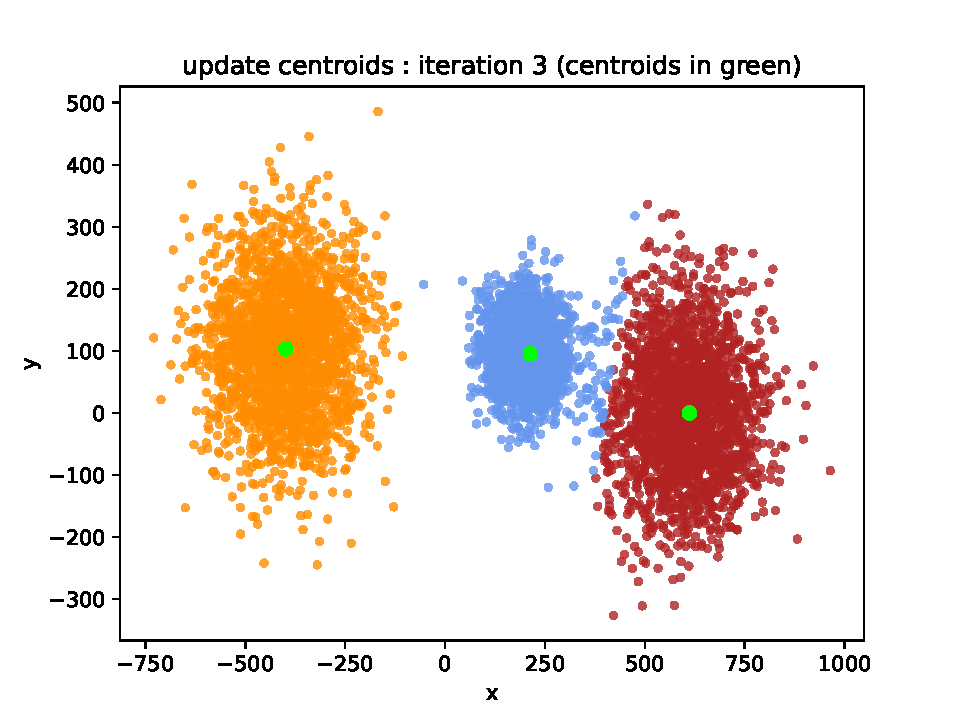
\includegraphics[width=8.5cm]{it_3_assign_samples_to_centroid}
\caption{}
\label{figure}
\end{figure}
\end{frame}

\begin{frame}
\frametitle{K-means}
\begin{figure}[!h]
\centering
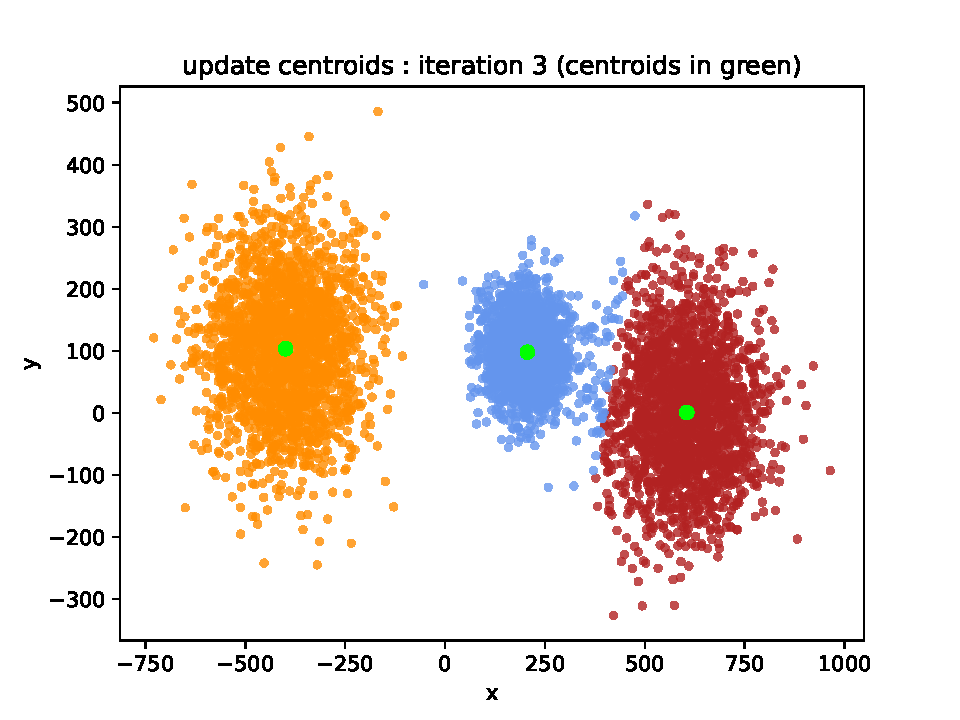
\includegraphics[width=8.5cm]{it_3_move_centroids}
\caption{Centroids 1st iteration}
\label{figure}
\end{figure}
\end{frame}


\begin{frame}{K-means and initialization}
    Note that when launching the algorithm several times, the result may
    differ. \textbf{{Why ?}} 
\end{frame}

\begin{frame}{K-means optimization problem}
    \begin{itemize}
        \item When performing the k-means algorithm, we optimize the \textbf{{inertia}}.
        \item if we have $n$ points, $x_i$, each assigned to a centroid $c_i$.
    \end{itemize}

   \begin{equation}
       I= \sum^{n}_{i=1} d(x_i,c_i)^2
   \end{equation}
   
   \begin{equation}
       I= \sum^{n}_{i=1} ||x_i- c_i||_2^2
   \end{equation}
   $||$ stands for "norm".
\end{frame}

\begin{frame}
\frametitle{K-means : Expectation Maximisation algorithm}
\begin{itemize}
	\item What could we do if the algorithm falls in a local optimum ?
\end{itemize}
\begin{figure}[htpb]
    \centering
    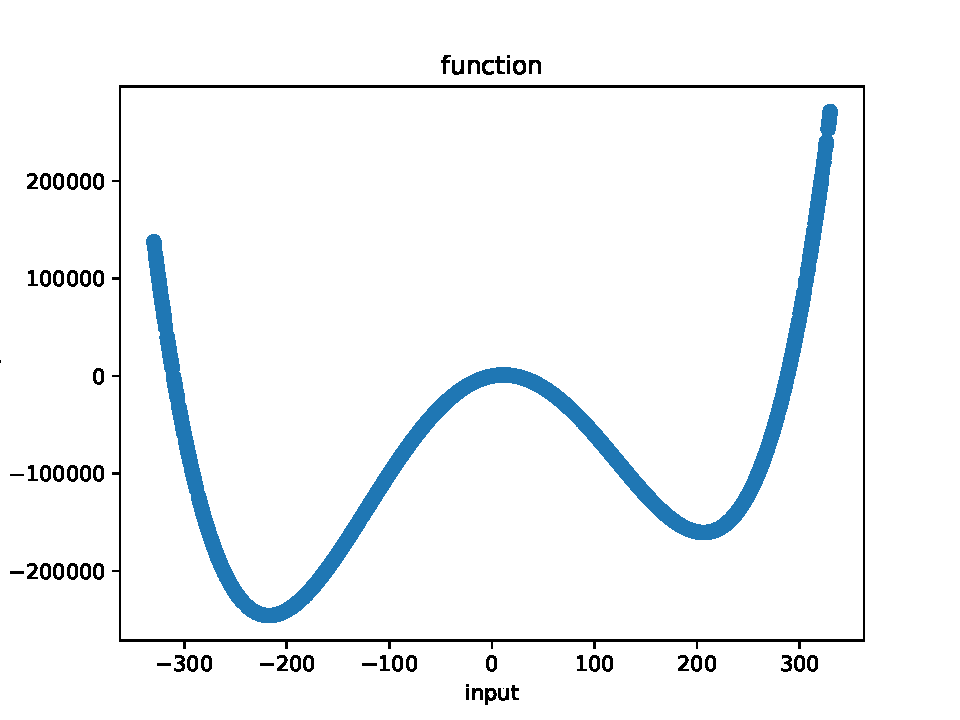
\includegraphics[width=0.4\linewidth]{function}
    \label{fig:function}
\end{figure}    
\end{frame}


\begin{frame}
    \exercice{} Perform the algorithm on the same dataset with scikit-learn (use the file: \textbf{k\textunderscore means\textunderscore sklearn.py})

    \begin{itemize}
        \item Observe the randomness of the result
        \item Explore the available parameters:

            \url{https://scikit-learn.org/stable/modules/generated/sklearn.cluster.KMeans.html} and find a solution in order to observe a \textbf{stable} result.
    \end{itemize}
    \begin{figure}[htpb]
        \centering
        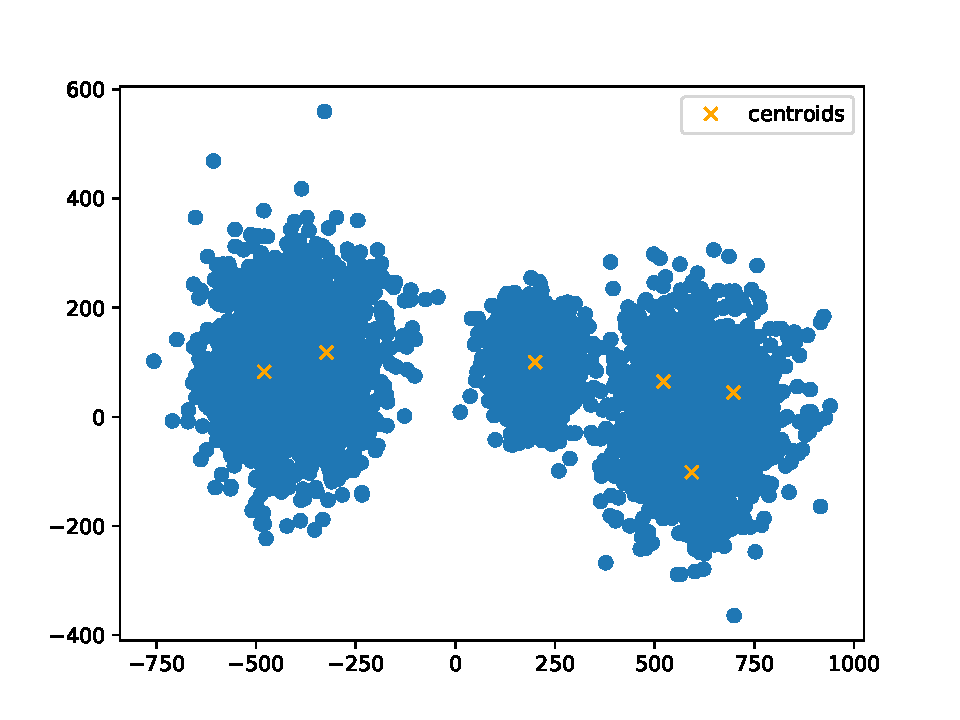
\includegraphics[width=0.4\linewidth]{sklearn_centroids}
        \label{fig:sklearn_centroids}
    \end{figure}
\end{frame}

\begin{frame}{Knee/elbow criterion}
    \begin{itemize}
        \item We would like a \textbf{{heuristic method}} in order to be able to assess a relevant number of clusters.
    \end{itemize}
\end{frame}

\begin{frame}{Knee/elbow criterion}
    \begin{itemize}
        \item \exercice{} use the file
            \textbf{{k\textunderscore means\textunderscore inertia.py}} in
            order to find a relevant number of clusters for the
            \textbf{{data\textunderscore 3D.npy}}, whith scikit-learn and kneed.

            \url{https://github.com/arvkevi/kneed}

	    Observe the behavior of this method when you run it on a different
            input dataset (you can generate a new one).
    \end{itemize}
\end{frame}

\begin{frame}{}
    \url{https://scikit-learn.org/stable/auto_examples/cluster/plot_kmeans_assumptions.html} 
\end{frame}


\section{Hierarchical clustering}
\frame{\tableofcontents[currentsection]}

\begin{frame}{Hierarchies}
    It is possible to perform a clustering in a hierarchical way. This means building a \textbf{sequence of clusterings}.

    \url{https://scikit-learn.org/stable/auto_examples/cluster/plot_agglomerative_dendrogram.html} 

    \url{https://docs.scipy.org/doc/scipy/reference/cluster.hierarchy.html} 
\end{frame}

\begin{frame}{Example application of hierarchical clustering}
    \begin{figure}[htpb]
        \centering
        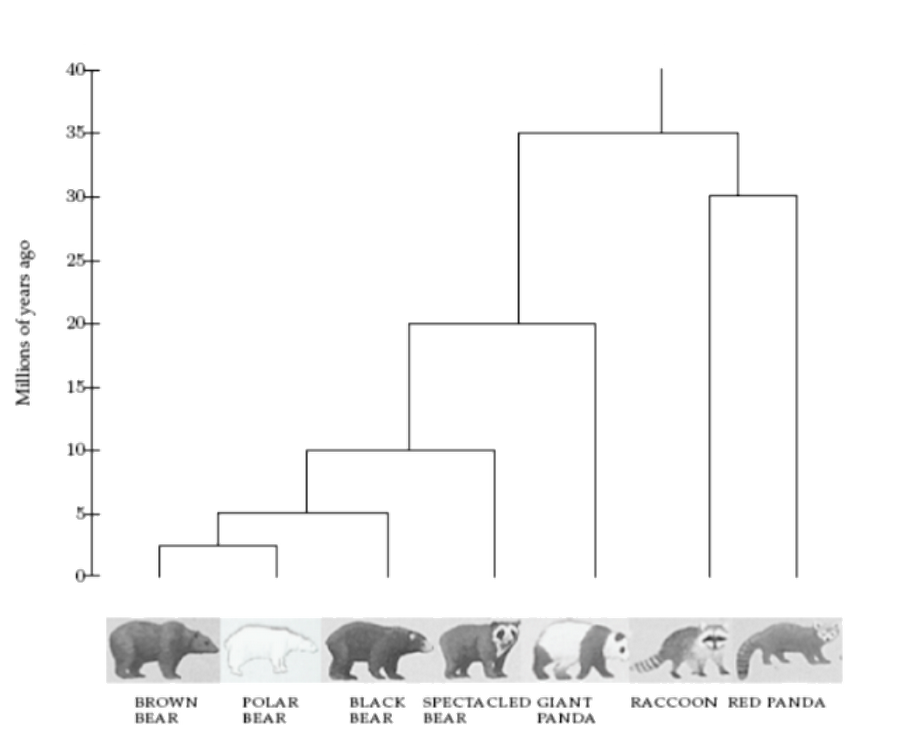
\includegraphics[width=0.6\linewidth]{hierarchy}
        \caption{ \url{https://towardsdatascience.com/hierarchical-clustering-and-its-applications-41c1ad4441a6} }
        \label{fig:name}
    \end{figure}
\end{frame}

\begin{frame}{Hierarchical clustering}
    We will apply hierarchical clustering to a small example dataset containing addresses.
\end{frame}


\begin{frame}{Hierarchical clustering}
   \exercice{\textbf{Plotting data}}

   \textbf{{cd hierarchical\textunderscore clustering/}} and use
    \textbf{{hierarchical\textunderscore clustering.py}} in order to show the
    scatter plot of the data (nuage de points) loaded from \textbf{{addresses.csv}}.

    Seaborn lib:
   \url{https://seaborn.pydata.org/}  
\end{frame}

\begin{frame}{Hierarchical clustering}
\begin{figure}[htpb]
    \centering
    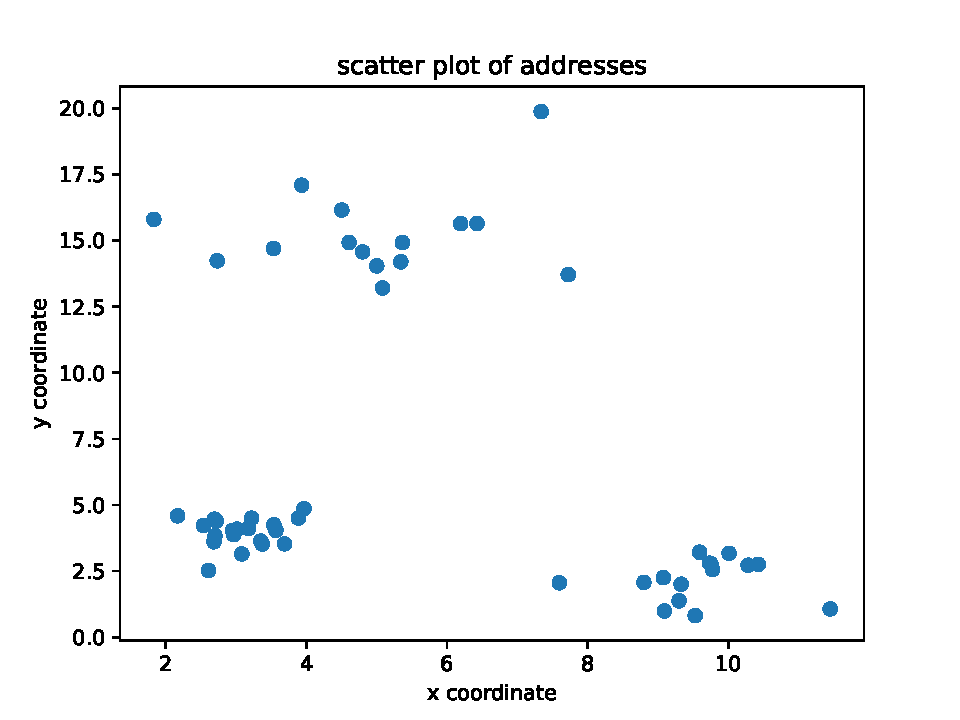
\includegraphics[width=0.6\linewidth]{scatter_plot_manual_2}
    \label{fig:scatter_plot_manual}
\end{figure}    
Hierarchical clustering consists in progressively grouping points together in
    \textbf{{classes.}} 
\end{frame}


\begin{frame}{Hierarchical clustering}
   \exercice{} Edit \textbf{{find\textunderscore closest\textunderscore classes()}} in order to find the closest classes. Then they can be merged in the while loop.
\end{frame}

\begin{frame}
    \begin{figure}[htpb]
        \centering
        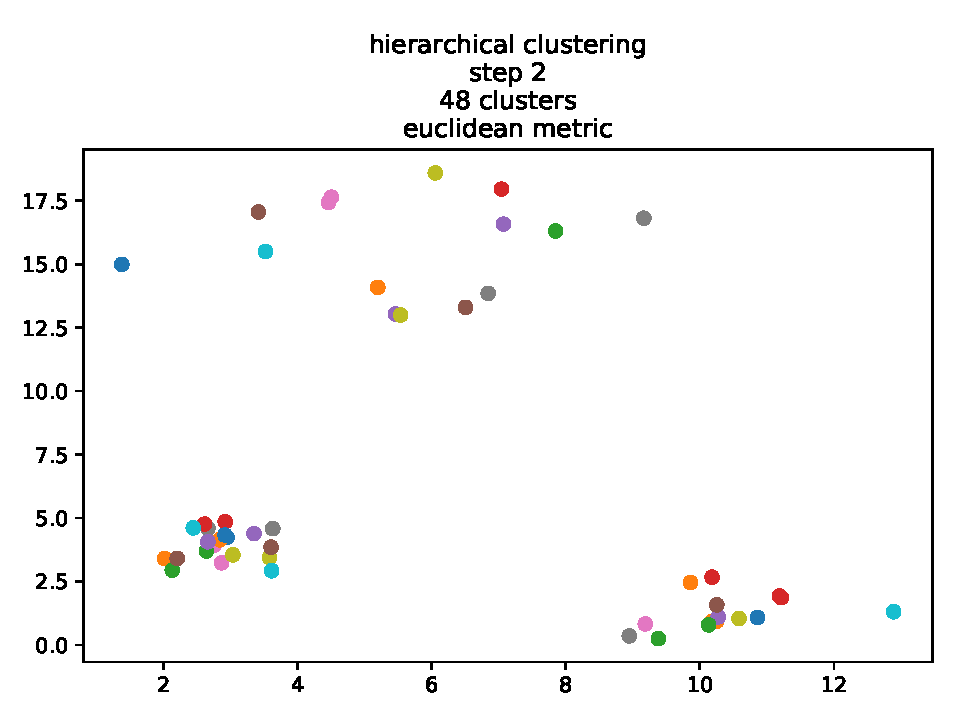
\includegraphics[width=0.8\linewidth]{clustering/clustering_step_2}
        \label{fig:clustering/clustering_step_2}
    \end{figure}
    
\end{frame}

\begin{frame}
    \begin{figure}[htpb]
        \centering
        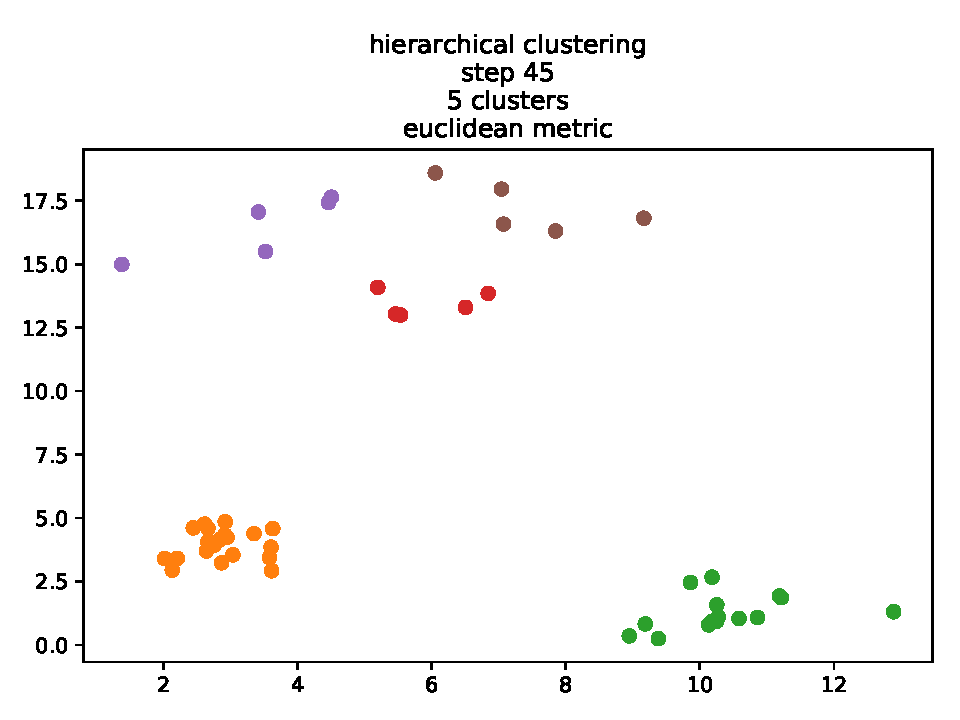
\includegraphics[width=0.8\linewidth]{clustering/clustering_step_45}
        \label{fig:clustering/clustering_step_2}
    \end{figure}
    
\end{frame}


\begin{frame}
    \begin{figure}[htpb]
        \centering
        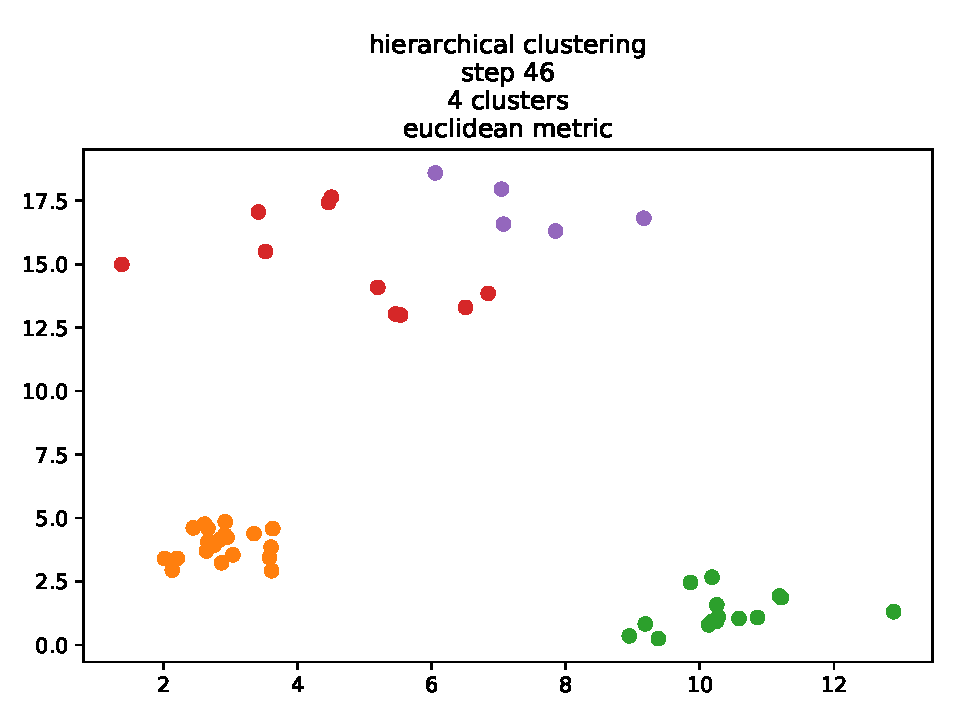
\includegraphics[width=0.8\linewidth]{clustering/clustering_step_46}
        \label{fig:clustering/clustering_step_2}
    \end{figure}
    
\end{frame}


\begin{frame}
    \begin{figure}[htpb]
        \centering
        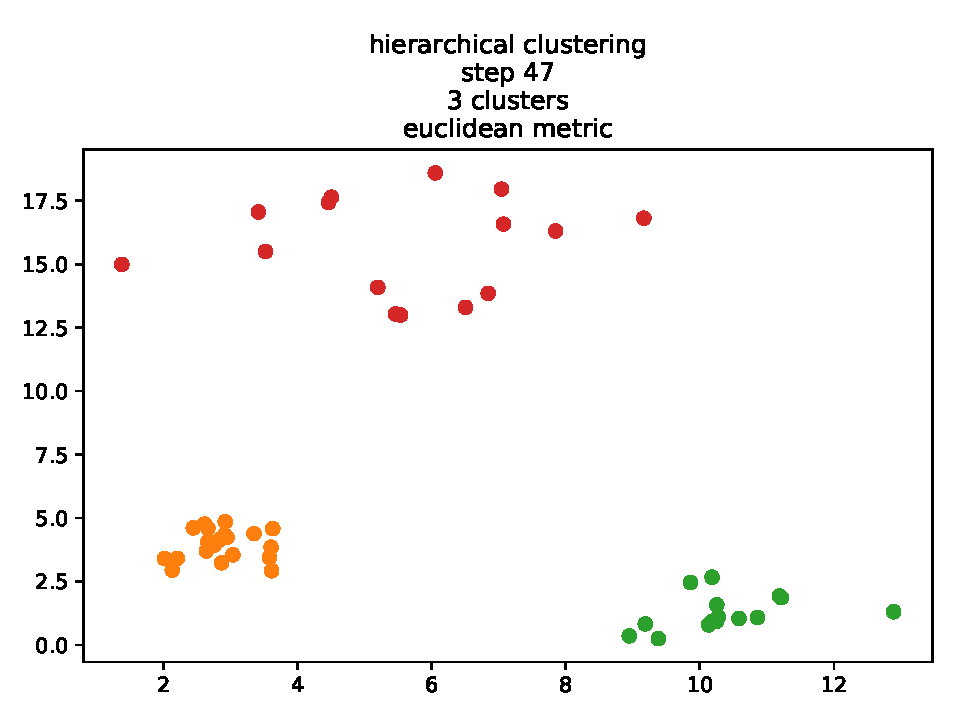
\includegraphics[width=0.8\linewidth]{clustering/clustering_step_47}
        \label{fig:clustering/clustering_step_2}
    \end{figure}
    
\end{frame}

\begin{frame}
    \begin{figure}[htpb]
        \centering
        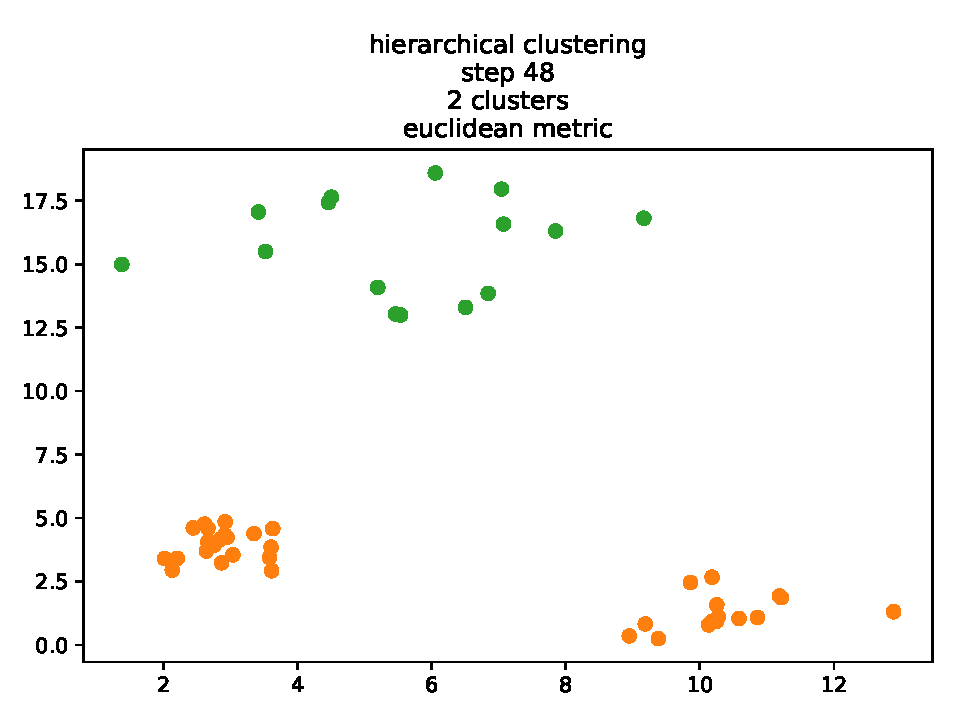
\includegraphics[width=0.8\linewidth]{clustering/clustering_step_48}
        \label{fig:clustering/clustering_step_2}
    \end{figure}
    
\end{frame}

\begin{frame}
    \begin{figure}[htpb]
        \centering
        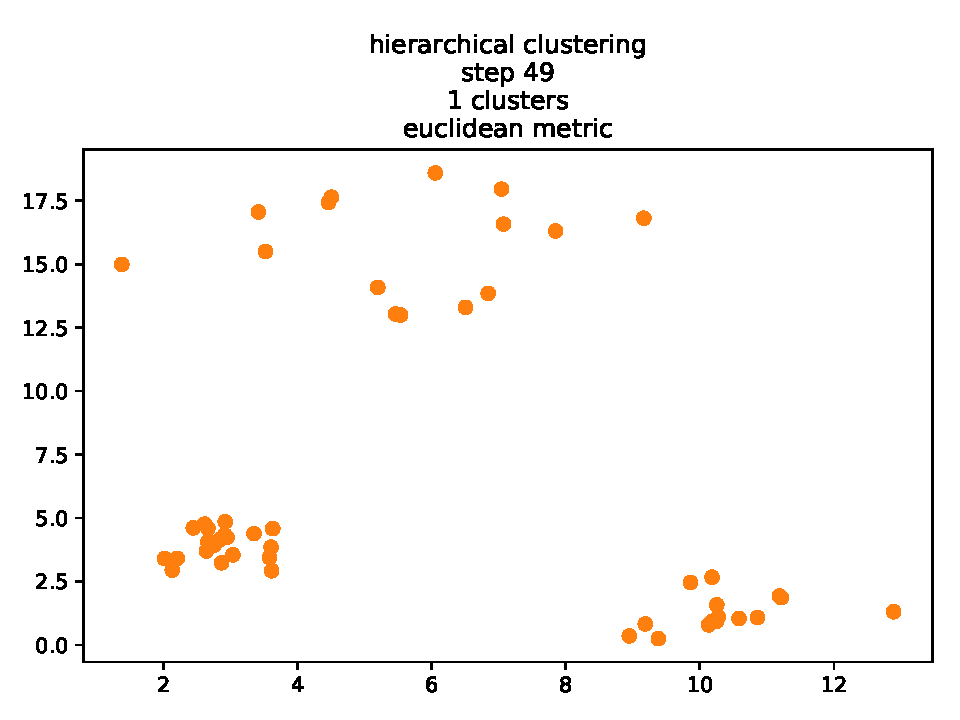
\includegraphics[width=0.8\linewidth]{clustering/clustering_step_49}
        \label{fig:clustering/clustering_step_2}
    \end{figure}
\end{frame}

\begin{frame}{Hierarchical clustering}
    An important  aspect of hierarchical clustering is that different criteria
    can be used in order to merge the classes. The distance between class 1 and class 2 can for instance be:
    \begin{itemize}
        \item the minimum distance between one point of class 1 and one point of class 2: \textbf{{single-linkage clustering}}.
	\item the average distance between points a class 1 and points a class 2: \textbf{{unweighted average linkage clustering}}
    \end{itemize}
    The two methods can lead to a different hierarchy of clusters.
    
\end{frame}

\begin{frame}{Average-linkage clustering}
    \exercice{Modify the computation of the distance between classes using the average-linkage criterion.}
\end{frame}

	\begin{frame}{Silhouette score}
	The Silhouette score is another heuristic used in order to choose a relevant number of clusters. File: \textbf{hierarchical\textunderscore clustering\textunderscore silhouette.py}.
	
	\begin{figure}[htpb]
		\centering
		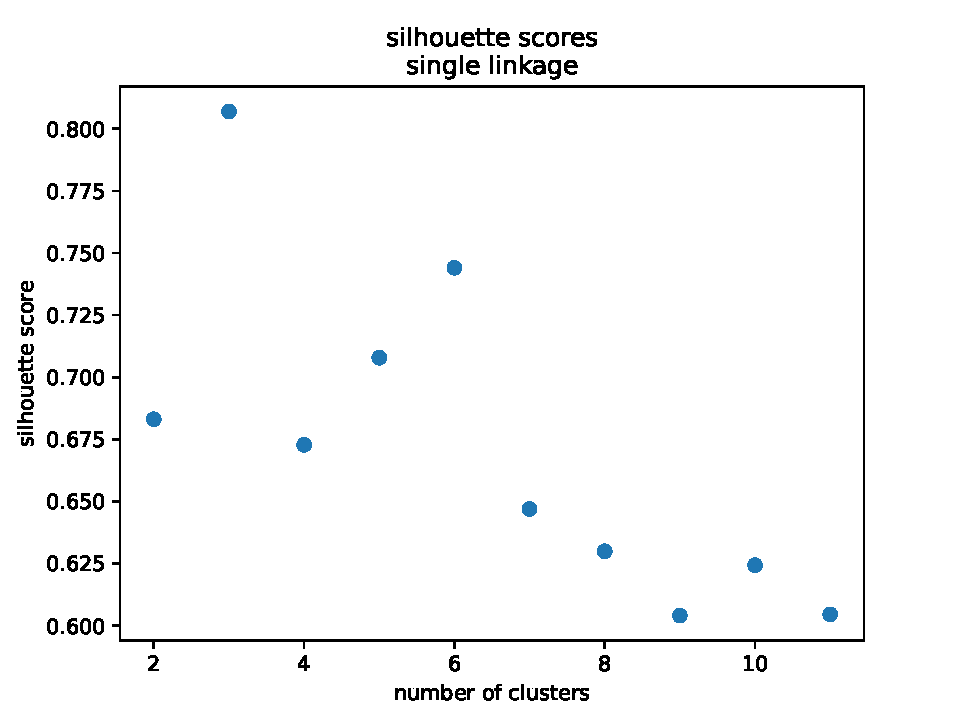
\includegraphics[width=0.6\textwidth]{silhouette_scores_single_linkage}
		\label{fig:silhouette_scores_single_linkage-pdf}
	\end{figure}
	\end{frame}


\section{Spectral clustering}
\frame{\tableofcontents[currentsection]}

\begin{frame}{Similarities}
    \begin{itemize}
        \item When working with distances, two points that "look the same" should be separated by a \textbf{{small distance}}.
	\item When working with a similarity, two points that "look the same" should have a \textbf{{high similarity}}. 
	\item Example: \textbf{adjacency relationship} in a graph: if $i$ and $j$ are related by an edge, $S_{ij}=1$, otherwise $S_{ij}=0$.
    \end{itemize}
\end{frame}

\begin{frame}{Adjacency matrix}
    \begin{figure}[htpb]
        \centering
        
\includegraphics[width=0.8\linewidth]{adjacency_matrix}
        \label{fig:name}
    \end{figure}
\end{frame}

\begin{frame}{Similarities}
    Differences between similarities and distances:
\begin{itemize}
    \item A similarity  $S$ is not always symmetrical.
    \item Indeed, in a \textbf{{directed graph}}, having a directed edge between $i$ and $j$ does not mean that we have an edge between $j$ and $i$.
    \item $S_{ij}=0$ does not mean that $i=j$, it is rather the contrary.
\end{itemize}    
\end{frame}

\begin{frame}{Similarities}
    \begin{itemize}
        \item A similarity is a more general notion than a distance. Given a similarity between two points, we can deduce a similarity.
	\item For instance this way, if $d_{ij}$ is the distance betwwen $i$ and $j$ : 
	    \begin{equation}
		S_{ij}=\exp(-d_{ij}) 
	    \end{equation}
    \end{itemize}
\end{frame}

\begin{frame}{Spectral Clustering}
    \begin{itemize}
        \item A clustering method that works with similarities
	\item It performs a low dimensional embedding of the similarity matrix, followed by a Kmeans 
    \end{itemize}
\end{frame}

\begin{frame}{Exercise}
    We will perform Spectral Clustering on this graph : 
    \begin{figure}[htpb]
        \centering
        
\includegraphics[width=0.6\linewidth]{graph_to_cluster}
        \label{fig:name}
    \end{figure}
\end{frame}


\begin{frame}
    \begin{figure}[htpb]
        \centering
        
\includegraphics[width=0.5\linewidth]{graph_to_cluster}
        \label{fig:name}
    \end{figure}
    \textbf{{cd spectral\textunderscore clustering/}} and use
    \textbf{{vanilla\textunderscore spectral\textunderscore clustering.py}} in
    order to apply spectral clustering. You first need to input the right
    \textbf{{affinity matrix}} or \textbf{{similarity matrix}} and then use the
    \textbf{{scikit-learn}} library. 
    \textbf{{doc}} : check the scikit page for Spectral Clustering.
\end{frame}


\begin{frame}{Spectral clustering}
    Some drawbacks of the method:
    \begin{itemize}
        \item Need to provide the number of clusters.
	\item Not adapted to a large number of clusters.
	\item kmeans step : so depends on a random initialization.
    \end{itemize}
\end{frame}


\subsubsection{Evaluating the quality of clustering} % (fold)
\label{ssub:evaluating_the_quality_of_clustering}

\begin{frame}{Heuristic}
    \begin{itemize}
        \item We would like a critetion in order to justify the number of clusters used.
    \end{itemize}
\end{frame}

\begin{frame}{Normalized cut : a measurement of the quality of a clustering}
    \begin{itemize}
	\item The \textbf{{cut of a cluster}} $C_k$, noted $Cut(C_k,V\backslash C_k)$ is the number of outside connections (connections with other clusters).
	\item The \textbf{{degree}} of a node is its number of adjacent edges
	\item The \textbf{{degree of a cluster}}, noted $d_{C_k}$ is the sum of the degrees of its nodes.
	\item The \textbf{{normalized cut}} of a clustering that contains $K$ clusters is:
	    \begin{equation}
NCut(\mathcal{C})=\sum_{k=1}^K\frac{Cut(C_k,V\backslash C_k)}{d_{C_k}}
	    \end{equation}

    \end{itemize}
\end{frame}

\begin{frame}{Normalization}
    \begin{itemize}
	\item The normalization is useful in order to take the \textbf{{weight}} (degree) of a cluster into account.
    \end{itemize}
\end{frame}


\begin{frame}{Normalized cut and clustering}
    Let's see how the normalized cut can help us choose the right number of clusters (backboard).
\end{frame}

\begin{frame}{Heuristic}
    \exercice{ \textbf{{Normalized but elbow:}} }

    Use \textbf{{normalized\textunderscore
    cut.py}} in order to estimate the relevant number of clusters in order to
    process the data contained in \textbf{{data/}}. These data are generated by
    \textbf{{generate\textunderscore data.py}}.
    \begin{figure}[htpb]
        \centering
        
\includegraphics[width=0.6\linewidth]{data_to_cluster}
        \label{fig:}
    \end{figure}
\end{frame}

\begin{frame}{Normalized cuts}
   \begin{figure}[htpb]
       \centering
       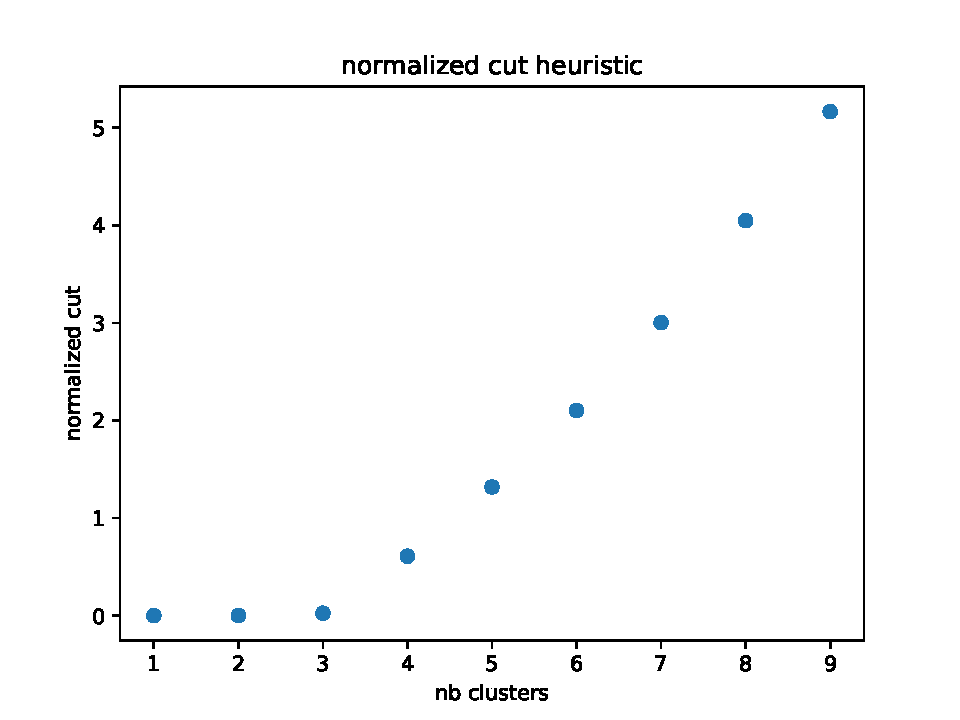
\includegraphics[width=0.8\linewidth]{cut}
       \label{fig:cut}
   \end{figure} 
\end{frame}

\begin{frame}{Normalized cuts}
   \begin{figure}[htpb]
       \centering
       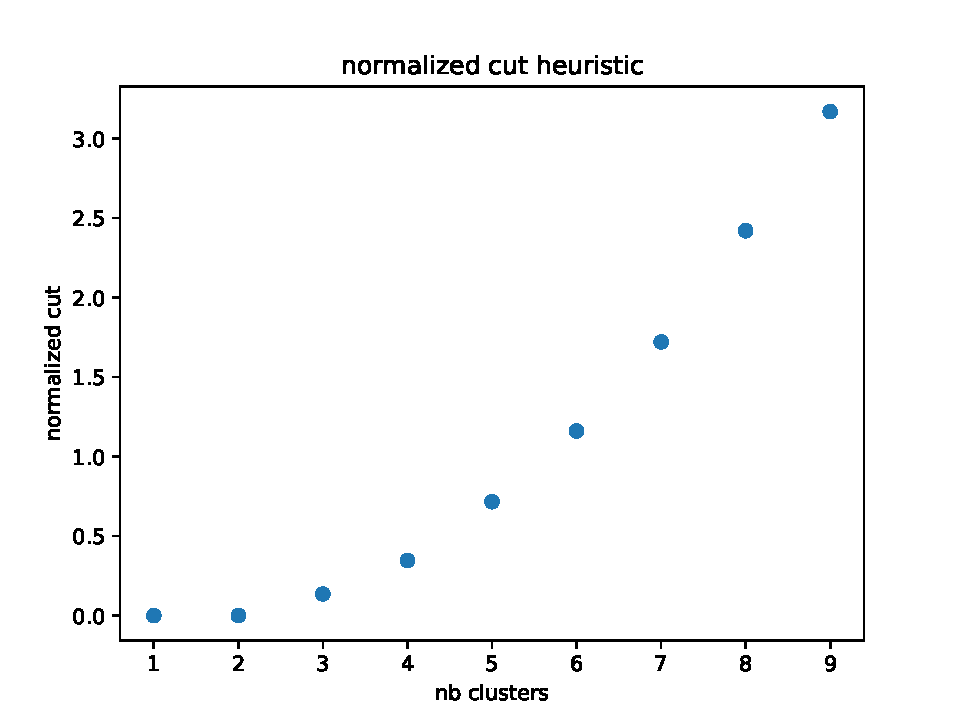
\includegraphics[width=0.6\linewidth]{spectral/normalized_cut_large_std}
       \caption{If the standard deviations in the dataset are larger, it is
       harder to identify a relevant number of clusters.}
       \label{fig:spectral/normalized_cut_large_std}
   \end{figure} 
\end{frame}


\begin{frame}{Similarity}
   \begin{figure}[htpb]
       \centering
       
\includegraphics[width=0.8\linewidth]{similarity}
       \label{fig:similarity}
   \end{figure} 
\end{frame}

\begin{frame}
\frametitle{Example}
\begin{figure}[!h]
\centering
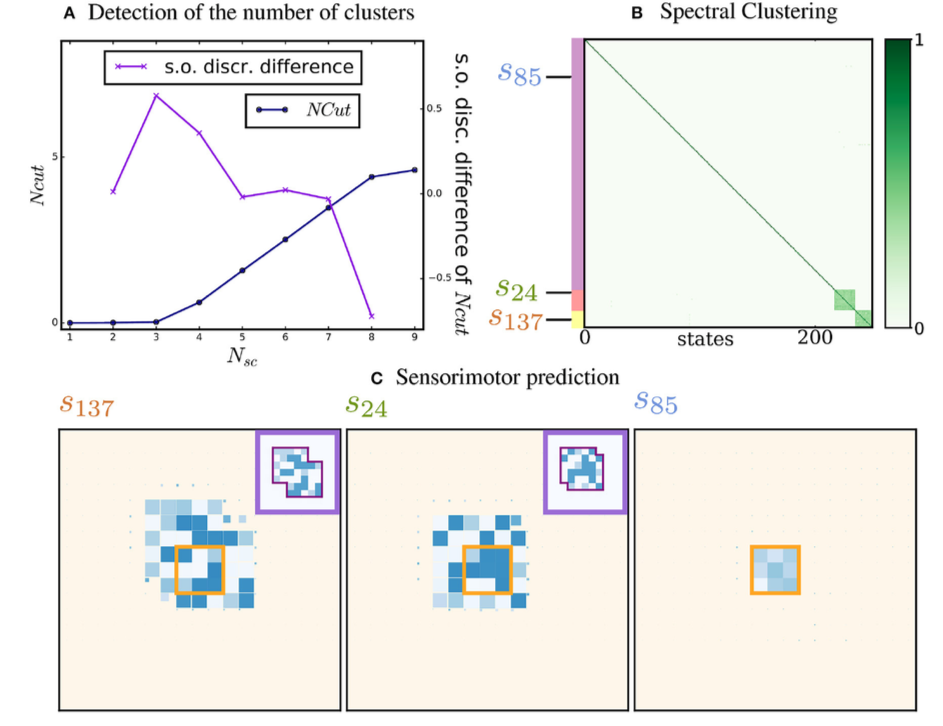
\includegraphics[width=7.5cm]{papier.png}
\caption{In a), the elbow method is used to choose the number of clusters. \cite{LeHir2018}}
\label{figure}
\end{figure}
\end{frame}


%\begin{frame}{Ressources on Spectral Clustering}
%    \begin{itemize}
%	\item \url{https://scikit-learn.org/stable/modules/generated/sklearn.cluster.SpectralClustering.html#sklearn.cluster.SpectralClustering} 
%        \item \url{https://scikit-learn.org/stable/auto examples/cluster/plot segmentation toy.html#sphx-glr-auto-examples-cluster-plot-segmentation-toy-py} 
%    \end{itemize}
%\end{frame}


\begin{frame}
\frametitle{Other methods to evaluate the quality of a clustering}
\begin{itemize}
	\item	Stability of the result when lauching the algorithm many times
	\item	Separation of the clusters (the mean distance between pairs of centroids is large)
	\item Ratio inter / intra
	\item Silhouette coefficient
\end{itemize}

\url{https://scikit-learn.org/stable/modules/clustering.html} 
\end{frame}

\begin{frame}
    \exercice{}

    Study the silouhette score as a function of the number of clusters for the
    hierarchical clustering problem.

    \url{https://scikit-learn.org/stable/modules/generated/sklearn.metrics.silhouette_score.html} 

\end{frame}

\begin{frame}{Silhouette coefficient with single linkage}
    \begin{figure}[htpb]
    	\centering
    	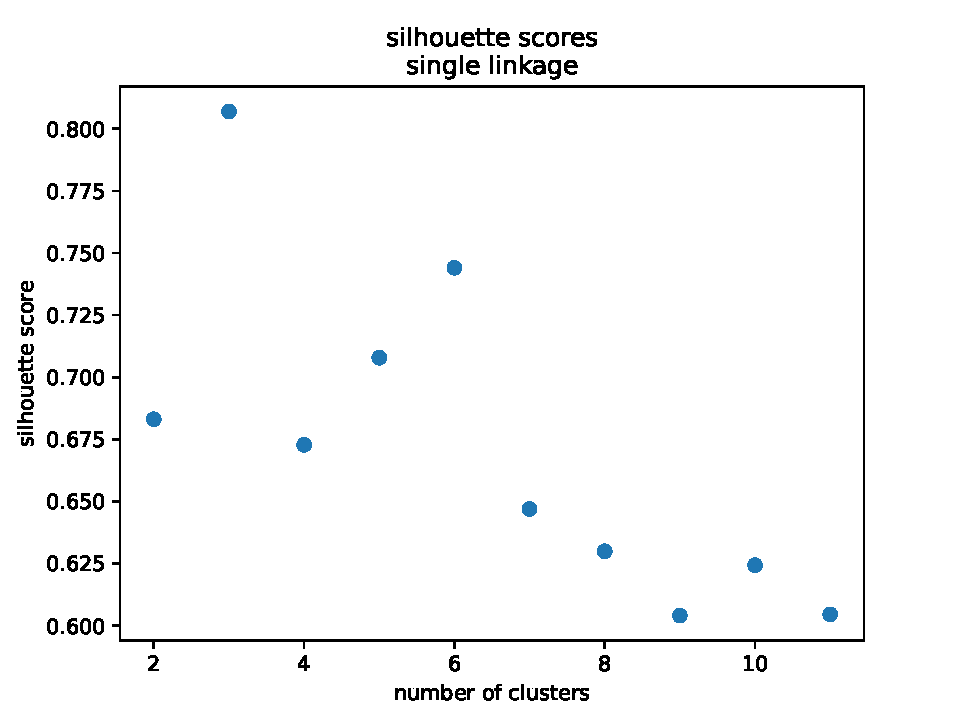
\includegraphics[width=0.8\textwidth]{silhouette_scores_single_linkage}
    \end{figure}
\end{frame}

\begin{frame}{Silhouette coefficient with average linkage}
    \begin{figure}[htpb]
    	\centering
    	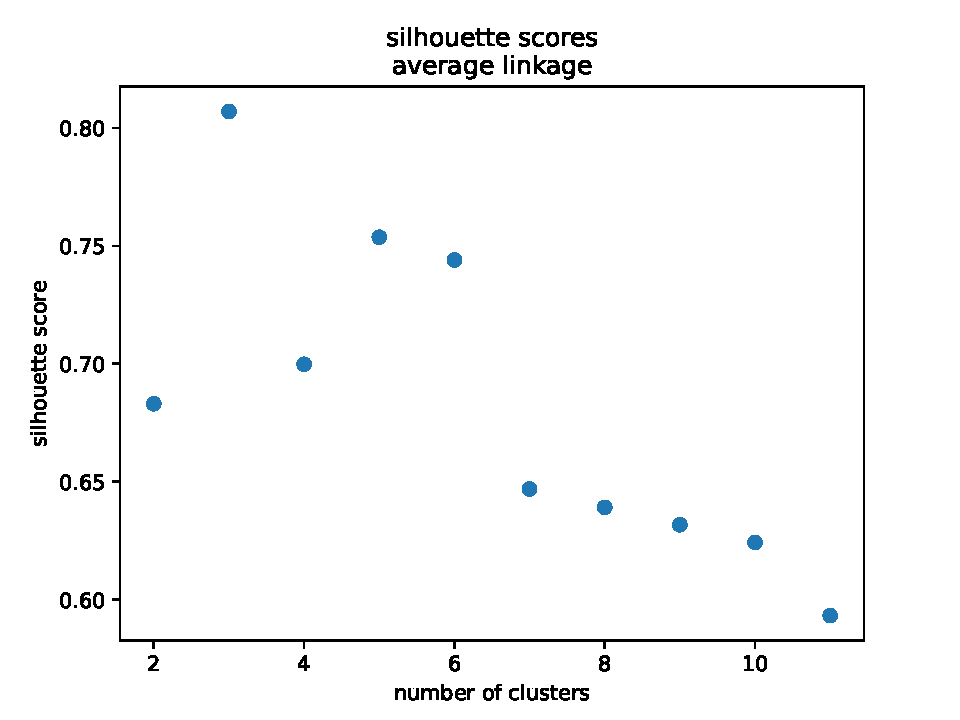
\includegraphics[width=0.8\textwidth]{silhouette_scores_average_linkage}
    \end{figure}
\end{frame}


\begin{frame}[allowframebreaks]
\frametitle{References}
\bibliographystyle{apalike}
\bibliography{epitech.bib} 
\end{frame}

\end{document} 
